% Windows: протестировано для MikTeX+TeXworks в режиме pdfLatex.
%
% Linux:
% Для получения pdf используйте команду  pdflatex rfa_2021.tex.
% Команда latex rfa_2021.tex выведет сообщение об ошибке.
%
\NeedsTeXFormat{LaTeX2e}
\documentclass[10pt,a4paper]{book}
\usepackage{NumMet_2024}
%--- Здесь можно вставить необходимые стили ---
% \usepackage{...}
%
%--- Здесь можно добавить свои команды --------
% \newcommand{}
\newcommand{\ceq}{\mathrel{\vcenter{\hbox{:=}}}}
%----------------------------------------------
\selectlanguage{russian}
\begin{document}
%===========================  ШАПКА СТАТЬИ =================================
\Article{Правила публикации и рекомендации к оформлению статей\break
    в журнале ``Вычислительные методы и программирование''}
    {Rules of publication and recommendations for formatting of articles 
    for the journal ``Numerical methods and programming''}
    
    \Abstract{Целью работы является разработка и анализ метода Гаусса–Зейделя с красно-черным упорядочиванием узлов трёхмерной равномерной расчётной сетки (Red-Black Gauss–Seidel, RBGS) для численного решения эллиптических уравнений с переменным коэффициентом на графическом ускорителе (GPU) с применением технологии NVIDIA CUDA. Расчётной областью для простоты выбран трёхмерный куб. Предложена адаптация RBGS под сеточные структуры и архитектуру CUDA с оптимизацией доступа к памяти. Выполнена конечно-разностная дискретизация эллиптического уравнения с переменным коэффициентом на трё равномерной сетке, параллельная реализация на GPU с использованием shared memory, сравнение с последовательной CPU-версией и методом Якоби.
    Вычислительный эксперимент подтвердил корректность разработанного алгоритма. На вычислительной системе с GPU ?????????? достигнуто ускорение до ???? на GPU по сравнению с CPU ???????? для сеток размером 1024 × 1024 × 1024 . Добавить анализ эффективности в зависимости от размера сетки и неоднородности коэффициента.}
    {The text describes the thematic focus of the journal, criteria 
    for selection of articles for publication, rules of submission of 
    articles for publication, the reviewing procedure, interaction of 
    authors with the editors. It also contains a style sheet with samples, 
    as well as rules of bibliographical descriptions both in Russian 
    and English.}

\Keywords{вычислительные методы и программирование, 
        журнал, 
        правила публикации.}
        {numerical methods and programming, 
        journal, 
        publishing rules.}

\Acknowledgements{Исследование выполнено за счет гранта Российского научного фонда № 22-71-10102-П, https://rscf.ru/project/22-71-10102/.}
    {The work was supported by the Russian Science Foundation (grant No. 22-71-10102-П, https://rscf.ru/project/22-71-10102/).}

\Citation{Писатель Е.Н.
    Правила публикации и рекомендации к оформлению статей
    в журнале ``Вычислительные методы и программирование''~//
    Вычислительные методы и программирование. 2021.
    \textbf{??}, \No~?. \pageref*{firstPage}--\pageref*{LastPage}.  
    doi 10.26089/NumMet.v??r???.}
    {Ye.~N.~Peesatel',
    ``Rules of publication and recommendations for formatting of articles 
    for the journal ``Numerical methods and programming,''
    Numerical Methods and Programming. \textbf{??} (?), 
    \pageref*{firstPage}--\pageref*{LastPage} (2021).
    doi~10.26089/NumMet.v??r???.}


\UDC{<указывает автор>}
\DOI{10.26089/NumMet.v??r???}% заполняет редакция
\VOL{??}{?}
\YEAR{2021}
\Received{16 июня 2021 г.}{June 16, 2021}
\Accepted{13 октября 2021 г.}{October 13, 2021}


\Author{Е.~Н.~Писатель}{Yevgraf~N.~Peesatel'}
\FullName{Евграф Никанорович Писатель}{Yevgraf~N.~Peesatel'}
% Место работы 1
\Institution{Московский государственный университет им. М. В. Ломоносова,\break 
Научно-исследовательский вычислительный центр}
{Lomonosov Moscow State University, Research Computing Center}
\Address{Ленинские горы, 1, стр.~4}{Leninskie Gory, 1, building 4}
\Postcode{119991}
\City{Москва}{Moscow}
\CountryOfResidence{Российская Федерация}{Russia}
% Место работы 2 (пример оформления)
%\Institution[2]{Национальная научная лаборатория им.~А.~Алиханяна (ЕрФИ)}{Alikhanyan National Science Laboratory (YerPhI)}
%\Address[2]{ул.~братьев Алиханян, д.~2}{Alikhanyan Brothers ulitsa, 2}
%\Postcode[2]{0036}
%\City[2]{Ереван}{Yerevan}
%\CountryOfResidence[2]{Армения}{Armenia}

\AcademicDegree{к.ф.-м.н.}{Ph.D.}
\Position{вед. научн. сотр.}{Leading Scientist}
\Orcid{kkkk-llll-mmmm-nnnn}
\Email{journal@num-meth.ru}

\MakeArticleHeader
%========================= КОНЕЦ ШАПКИ СТАТЬИ ==============================

\pagebreak

\section{Введение}

\subsection{Актуальность проблемы}

Эллиптические уравнения с переменным коэффициентом описывают широкий класс физических процессов: стационарную теплопроводность неоднородных сред, фильтрацию в пористых средах, распределение электрического потенциала в неоднородных диэлектриках.

Для численного решения на крупных сетках прямые методы (например, LU-разложение) становятся непрактичными из-за вычислительной сложности O(N³), что делает итерационные методы предпочтительными.

Добавить краткий обзор итерационных методов со ссылками на статьи в высокоуровневых научных журналах и обоснование выбора метода Зейделя

Метод Зейделя имеет быструю сходимость (обычно в два раза быстрее метода Якоби), но в классической формулировке является последовательным из-за зависимости обновления узла от уже обновлённых соседей. Прямой перенос последовательного алгоритма на GPU приводит к существенным задержкам и неэффективному использованию ресурсов вычислительной системы.

Задачи:
\begin{enumerate}
    \item 
    Разработать параллельный алгоритм метода Зейделя с красно-черным упорядочиванием, учитывающий технические характеристики GPU и выполнить его программную реализацию.
    \item
    Получить аналитические оценки времени исполнения алгоритма.
    Провести серию вычислительных экспериментов для определения метрик производительности (ускорение и пр.).
    \item
    Сравнить разработанный алгоритм с альтернативными итерационными методами (метод Якоби, последовательная CPU-версия).
    \item
    Разработать алгоритм адаптивного выбора вычислителя (CPU или GPU) для решения сеточных уравнений на сетке с заданными параметрами.
    \item
    Разработать алгоритм выбора параметров расчётной сетки и конфигурации ядер CUDA на основе технических характеристик GPU.
\end{enumerate}

\section{Постановка задачи и дискретизация}

\subsection{Модельное уравнение}

Рассматривается стационарное уравнение диффузии:

$ -\nabla \cdot (a(x,y,z) \nabla u) = f(x,y,z), \quad (x,y,z) \in \Omega, $

с граничными условиями Дирихле u | $\partial$ $\Omega = g(x, y, z)$ .
Коэффициент $a (x, y, z) > 0$ – пространственно-переменный, непрерывный.

В работе используется расчётная область $\Omega = [0, L_x] × [0, L_y] × [0, L_z]$ в форме прямоугольного параллелепипеда.

\subsection{Конечно-разностная дискретизация}

Введём равномерную расчётную сетку $\omega$ $h = ( x_i , y_j , z_k ) : x_i = ih_x , ; y_j = jh_y ; z_k = kh_z$ с числом узлов $N = ( N_x + 1 ) × ( N_y + 1 )$ , где $h_x = L_x / N_x , h_y = L_y / N_y , h_z = L_z / N_z $.

Используем пятиточечный шаблон с аппроксимацией переменного коэффициента на гранях ячеек методом среднего арифметического:

$ -\frac{a_{i+1/2,j,k}(u_{i+1,j,k}-u_{i,j,k}) - a_{i-1/2,j,k}(u_{i,j,k}-u_{i-1,j,k})}{h_x^2} \\ - \frac{a_{i,j+1/2,k}(u_{i,j+1,k}-u_{i,j,k}) - a_{i,j-1/2,k}(u_{i,j,k}-u_{i,j-1,k})}{h_y^2} \\ - \frac{a_{i,j,k+1/2}(u_{i,j,k+1}-u_{i,j,k}) - a_{i,j,k-1/2}(u_{i,j,k}-u_{i,j,k-1})}{h_z^2} = f_{i,j,k}. $

В результате получим систему линейных алгебраических уравнений $A u = b$ с симметричной положительно определенной матрицей A (M-матрица).


\vspace*{4mm plus 2mm minus 2mm}
%=======================  Список литературы ==================================
%
% Команда \LITERRUS печатает "СПИСОК ЛИТЕРАТУРЫ" и обнуляет счетчики
%
\LITERRUS
% \rlitem{arg1}{arg2} --- создает пункт списка литературы.
% arg1 --- символическая ссылка на источник, используется при создании ссылки командой \ref
% arg2 --- текст, помещаемый в пункт списка. Может содержать команды выбора начертания 
%          символов и др.
\rlitem{rfa:rulit:COPE1}{
Guidelines on Good Publication Practice. Committee on Publication Ethics (COPE).
\url{https://publicationethics.org/files/u7141/1999pdf13.pdf}.
(Дата обращения: 12 ноября 2021).}

\rlitem{rfa:rulit:Kotelnikov}{
\textit{Котельников И.А., Чеботаев П.З.} \LaTeX\ по-русски. Новосибирск: 
Сибирский хронограф, 2004.}

\rlitem{rfa:rulit:Samarin}{
\textit{Гуссенс М., Миттельбах Ф., Самарин А.} Путеводитель по пакету \LaTeX\ и его
расширению \LaTeXe. М.: Мир, 1999.}

\rlitem{rfa:rulit:Lvovski}{
\textit{Львовский С.М.} Набор и верстка в системе \LaTeX. М.: МЦНМО, 2003.
}

\rlitem{rfa:rulit:rot}{
\textit{Бугров Я.С., Никольский С.М.} Высшая математика. Дифференциальные уравнения. Кратные интегралы.
Ряды. Функции комплексного переменного. Учебник для вузов. Ростов н/Д: Изд-во ``Феникс'', 1998.
}

\rlitem{rfa:rulit:Antonov}{
\textit{Антонов А.С.} Параллельное программирование с использованием технологии OpenMP. Учебное пособие.
М.: Изд-во МГУ, 2009.
}

\rlitem{rfa:rulit:Lapko}{
\textit{Лапко О.} Пакет makecell. \url{https://mirror.truenetwork.ru/CTAN/macros/latex/contrib/makecell/makecell-rus.pdf}.
(Дата обращения: 12 ноября 2021).}

\rlitem{rfa:rulit:mrow}{%
Multirow~--- Create tabular cells spanning multiple rows.
\url{https://www.ctan.org/pkg/multirow}.
(Дата обращения: 12 ноября 2021).}

%=======================  Список литературы ==================================
\medskip
\DateRU 

\medskip

\MakeAuthorsInfoRU

%===========================  REFERENCES =====================================
\pagebreak

\REFERENCES

\elitem{rfa:enlit:COPE1}{
Guidelines on Good Publication Practice. Committee on Publication Ethics (COPE).
\url{https://publicationethics.org/files/u7141/1999pdf13.pdf}.
Cited November 12, 2021.}

\elitem{rfa:enlit:Kotelnikov}{
I.~A.~Kotel'nikov and P.~Z.~Chebotaev, 
\textit{\LaTeX\ in Russian} 
(Sibirskiy Khronograph, Novosibirsk, 2004) [in Russian].}

\elitem{rfa:enlit:Samarin}{
M.~Goossens, F.~Mittelbach, and A.~Samarin, 
\textit{The \LaTeX~Companion.} 
(Addision--Wesley Professional, 1994; Mir, Moscow, 1999) 
[in Russian].}

\elitem{rfa:enlit:Lvovski}{
S.~M.~L'vovsky. \textit{Typesetting and Layout in the \LaTeX~System}
(MCNMO Publ., Moscow, 2003) 
[in Russian].}


\elitem{rfa:enlit:rot}{
Ya.~S.~Bugrov and S.~M.~Nikol'sky, 
\textit{Higher Mathematics: Differential Equations. Multiple Integrals. Ranks} 
(Phoenix Publ., Rostov-na-Donu, 1998) 
[in Russian].}

\elitem{rfa:enlit:Antonov}{
A.~S.~Antonov, 
\textit{Parallel Programming Using OpenMP Technology}
(Mosk. Gos. Univ., Moscow, 2009) 
[in Russian].}

\elitem{rfa:enlit:Lapko}{
O.~Lapko, 
\textit{The Makecell Package}. 
\url{https://mirror.truenetwork.ru/CTAN/macros/latex/contrib/makecell/makecell-rus.pdf}.
Cited November 12, 2021 [in Russian].}


\elitem{rfa:enlit:mrow}{%
Multirow~--- Create Tabular Cells Spanning Multiple Rows.
\url{https://www.ctan.org/pkg/multirow}.
Cited November~12, 2021.}


\medskip
\DateEN

\bigskip

\MakeAuthorsInfoEN

%\end{document}
%============================ КОНЕЦ СТАТЬИ ==================================



%============================ ПРИЛОЖЕНИЕ 1 ==================================
\newpage
\Appendix{Оформление листингов программ и алгоритмов}{pril:prog}


\textbf{Листинг~\ref{pril:prog:lst1}.~Программа на языке C/C++, занимающая всю ширину 
полосы набора.} Обращаем внимание авторов на следующую особенность окружения
\verb!\begin{lstlisting}...\end{lstlisting}!:
квадратные скобки \verb![! \verb!]! используются для задания блока параметров,
а запятая~\verb!,!~--- для разделения параметров. Заголовок листинга на русском и 
английском языках набран следующим образом:
\begin{verbatim}
caption={Пример оформления фрагмента программы 
         (с разрешения автора \mbox{[\ref{rfa:rulit:Antonov}]})},
bicaption={An example of the design of a program fragment 
           (with the permission of the author \mbox{[\ref{rfa:rulit:Antonov}]})},
\end{verbatim}
Внешние фигурные скобки в \verb!caption={...}! и в \verb!bicaption={...}!
позволяют использовать при необходимости запятую в тексте заголовка,
а конструкция \verb!\mbox{[\ref{rfa:rulit:Antonov}]}! экранирует
квадратные скобки \verb![! \verb!]!, позволяя использовать их в ссылке 
на источник.
%
% ЛИСТИНГ 1. ПРОГРАММА НА С
%
\begin{lstlisting}[%
      caption={Пример оформления фрагмента программы (с разрешения автора \mbox{[\ref{rfa:rulit:Antonov}]})},
      bicaption={An example of the design of a program fragment (with the permission of the author \mbox{[\ref{rfa:rulit:Antonov}]})},
      label=pril:prog:lst1,
      float=h!, % может быть t, h, b, t!, h!, b!
      language=C, 
      inputencoding=utf8, 
      extendedchars=\true, 
      keywordstyle=\color{blue!75!black}, 
      keepspaces=true, 
      commentstyle=\color{green!40!black}, 
      breakatwhitespace=true,
      frame=single, 
      linewidth=169mm,
      xleftmargin=7mm,
      basicstyle=\ttfamily\small,
      numbers=left,
      breaklines=\true, 
      numberstyle=\footnotesize,
      tabsize=8]
// OpenMP technology
// applying the single directive with the nowait option 
#include <stdio.h>

int main (int argc, char *argv[])
{
#pragma omp parallel
{
      printf("Message 1\n");
#pragma omp single nowait
      {
            printf("One thread\n");
      }
      printf("Message 2\n");
}
}
\end{lstlisting}

\textbf{Листинг~\ref{pril:prog:lst2}.~Программа на языке Fortran.} 
Полезным для авторов может оказаться параметр \verb!float!, который определяет
размещения листинга как плавающего объекта на странице: 
\verb+t+ и \verb+t!+ задают размещение в верхней части страницы, 
\verb+b+ и \verb+b!+~--- в нижней части, 
а \verb+h+ и \verb+h!+~--- в том месте текста, где расположен листинг.
Использование параметров с восклицательным знаком \verb+t!+, \verb+b!+ и
\verb+h!+ гарантирует, что листинг будет размещен на ближайшей возможной странице.
%
% ЛИСТИНГ 2. ПРОГРАММА НА FORTRAN
%
\begin{lstlisting}[%
      caption={Нераспределенный параллельный цикл в языке FDVMH (плавающий объект)},
      bicaption={Undistributed parallel loop in FDVMH language (floating object)},
      label={pril:prog:lst2},
      float=b!, % может быть t, h, b, t!, h!, b!
      language=Fortran, 
      inputencoding=utf8, 
      extendedchars=\true, 
      keywordstyle=\color{blue!75!black}, , 
      keepspaces=true, 
      commentstyle=\color{green!40!black}, 
      breakatwhitespace=true,
      frame=single, 
      linewidth=169mm,
      xleftmargin=7mm,
      basicstyle=\ttfamily\small,
      numbers=left,
      breaklines=true, 
      numberstyle=\footnotesize,
      tabsize=2]  
!DVM$ REGION TARGETS(HOST) OUT(A)
!DVM$ PARALLEL(I,J,K) TIE (A(K,J,I)) 
  DO I = Li, Hi
    DO J = Lj, Hj
      DO K = Lk, Hk
        A(K,J,I) = ....
!DVM$ END REGION       
\end{lstlisting}

\smallskip
\textbf{Алгоритм~\ref{pril:prog:alg1}.~Пример оформления алгоритма.} 
В существующих в \LaTeXe{} пакетах \verb!algorithm!, \verb!algpseudocode! и др. 
собраны различные команды и окружения, придающие алгоритмам вид, принятый в
западной научной литературе. Команды в этих пакетах определяют представление
алгоритмических операций: например, команда \verb!x\gets 10! отображается
в виде $x\leftarrow 10$ и означает присвоение переменной $x$ значения~10.

Нередко авторы нашего журнала, ввиду отсутствия отечественного стандарта в этой области,
используют оригинальные обозначения алгоритмических операций, поэтому 
редакция рекомендует для набора алгоритмов применять команды, определенные 
в стилевом файле журнала. В отличие от пакетов \verb!algorithm!, \verb!algpseudocode! и 
некоторых других, в нашем стилевом файле определены команды, которые отвечают за
размещение алгоритмических операций, но не за их представление.

Рассмотрим основные команды, которые использовались при наборе алгоритма \ref{pril:prog:alg1}.
Окружение 
\begin{verbatim}
\begin{nmAlgorithm}{<символическая метка>}
      {<заголовок на русском языке>}
      {<заголовок на английском языке>}
...
\end{nmAlgorithm}
\end{verbatim}
размечает область для алгоритма. Команда 
\begin{verbatim}
\algLine[<количество отступов>][<символическая метка>]{<алгоритмическая операция>}
\end{verbatim}
используется для формирования строки алгоритма. Параметры \verb!<количество отступов>!
и \verb!<символическая! \verb!метка>! являются необязательными для команды 
\verb!\algLine!. 

В стилевом файле для удобства определены команды для часто используемых
алгоритмических операций и конструкций:
\verb!\algINPUT!~--- печатает \textbf{input};
\verb!\algFOR!~--- \textbf{for};
\verb!\algDO!~--- \textbf{do};
\verb!\algENDFOR!~--- \textbf{end for};
\verb!\algIF!~--- \textbf{if};
\verb!\algTHEN!~--- \textbf{then};
\verb!\algELSE!~--- \textbf{else};
\verb!\algELIF!~--- \textbf{elseif};
\verb!\algENDIF!~--- \textbf{end if};
\verb!\algOUTPUT!~--- \textbf{output};
\verb!\algSTOP!~--- \textbf{stop};
\verb!\algFUNC!~--- \textbf{function};
\verb!\algENDFUNC!~--- \textbf{end function}.
Определение этих команд примитивно:\\ 
\hspace*{50mm}\verb!\newcommand{\algELSE}{\textbf{else\ }}!,\\
а их набор может быть раширен автором статьи в случае необходимости самостоятельно.

Определенная в стилевом файле команда\\ 
\hspace*{50mm}\verb!\algGOTO[1]{\textbf{goto}~\ref*{#1}}!\\
принимает в качестве аргумента символическую метку, указанную в команде \verb!\algLine!,
и формирует текст \textbf{goto\ }\verb!<номер строки, содержащей метку>!.

\begin{nmAlgorithm}{pril:prog:alg1}
      {Функция $g$ (вычисление координат точки $v$ по ее порядковому номеру $k$)}
      {Function $g$ (calculating the coordinates of the point $v$ by its ordinal $k$)}
     \algLine{\algFUNC $g(k,d,p)$}
     \algLine[1]{$u_{n-1} \ceq \left\lfloor k/\left(d-1\right)^{n-2}\right\rfloor$}
     \algLine[1]{$u_n \ceq u_{n-1}$}
     \algLine[1]{$k\ceq k\mod (d-1)^{n-2}$}
     \algLine[1]{\algFOR $j=\left(n-3\right)\ldots0$ \algDO}
     \algLine[2]{$u_j\ceq \left\lfloor k/(d-1)^j\right\rfloor+1$}
     \algLine[2]{$k\ceq k\mod(d-1)^j$}
     \algLine[1]{\algENDFOR}
     \algLine[1]{\textbf{return} $(v_1,\dots,v_n)$}
     \algLine{\algENDFUNC}
\end{nmAlgorithm}

\medskip
\textbf{Алгоритм~\ref{pril:prog:alg2}.~Сопоставление двух вариантов алгоритма.} 
Для того чтобы читателю было удобно сопоставлять варианты какого-либо алгоритма
или показать различие двух схожих алгоритмов, автору требуется разместить их 
построчно рядом друг с другом (см. алгоритм~\ref{pril:prog:alg2}).

Для набора алгоритмов, требующих сопоставления, нужно воспользоваться командой 
\begin{verbatim}
\algLineDouble[<количество отступов>][<символическая метка>]
      {<алгоритмическая операция, алгоритм 1>}{<алгоритмическая операция, алгоритм 2>},
\end{verbatim}
которая размещает строки алгоритмов в две колонки. 

\pagebreak
\begin{nmAlgorithm}{pril:prog:alg2}
      {Генерация точек валидационного множества (параметры $d, \rho$)}
      {Generating validation set points (parameters $d, \rho$)}
\algLineDoubleComment{а) с дубликатами \oppo{(with dublicates)}}{б) без дубликатов \oppo{(no dublicates)}}
\algLineDouble[0][a1:l1]{$\varphi := \pi/d$}{$\varphi := \pi/d$}
\algLineDouble[0][a1:l2]{\algFOR $j_{n-1} = 0\ldots (2d-1)$ \algDO}{\algFOR $j_{n-1} = 0\ldots (2d-1)$ \algDO}
\algLineDouble[1]{$\theta := j_{n-1}\varphi$}{$\theta := j_{n-1}\varphi$}
\algLineDouble[1]{\algFOR $j_{n-2} = 0\ldots d$ \algDO}{\algFOR \corr{$j_{n-2} = 1\ldots d-1$} \algDO}
\algLineDouble[2]{$\phi_{n-2} := j_{n-2}\varphi$}{$\phi_{n-2} := j_{n-2}\varphi$}
\algLineDouble[2]{\ldots}{\ldots}
\algLineDouble[2]{\algFOR $j_2 = 0\ldots d$ \algDO}{\algFOR \corr{$j_2 = 1\ldots d-1$} \algDO}
\algLineDouble[3]{$\phi_2 := j_1\varphi$}{$\phi_2 := j_1\varphi$}
\algLineDouble[3]{\algFOR $j_1 = 0\ldots d$ \algDO}{\algFOR \corr{$j_1 = 1\ldots d-1$} \algDO}
\algLineDouble[4]{$\phi_1 := j_1\varphi$}{$\phi_1 := j_1\varphi$}
\algLineDouble[4]{$\varpi := 1$}{$\varpi := 1$}
\algLineDouble[4]{$v_1 := \rho \cos(\phi_1)$}{$v_1 := \rho \cos(\phi_1)$}
\algLineDouble[4]{\algFOR $l=2\ldots n-2$ \algDO}{\algFOR $l=2\ldots n-2$ \algDO}
\algLineDouble[5]{$\varpi := \sin(\phi_{l-1})\varpi$}{$\varpi := \sin(\phi_{l-1})\varpi$}
\algLineDouble[5]{$v_l := \rho\cos(\phi_l)\varpi$}{$v_l := \rho\cos(\phi_l)\varpi$}
\algLineDouble[4]{\algENDFOR }{\algENDFOR }
\algLineDouble[4]{$v_{n-1} := \rho\sin(\theta)\varpi$}{$v_{n-1} := \rho\sin(\theta)\varpi$}
\algLineDouble[4]{$v_n := \rho\cos(\theta)\varpi$ }{$v_n := \rho\cos(\theta)\varpi$ }
\algLineDouble[4]{\algOUTPUT $v$}{\algOUTPUT $v$}
\algLineDouble[3]{\algENDFOR}{\algENDFOR}
\algLineDouble[2]{\algENDFOR}{\algENDFOR}
\algLineDouble[2]{\ldots}{\ldots}
\algLineDouble[1]{\algENDFOR}{\algENDFOR}
\algLineDouble{\algENDFOR}{\algENDFOR}
\algLineDouble{\algSTOP}{\algSTOP}\par
\end{nmAlgorithm}
      
\medskip
\textbf{Алгоритм~\ref{pril:prog:alg3}.~Пример совмещения текста статьи и алгоритма.} 
Ниже приведен пример оформления небольшого алгоритма рядом с текстом статьи.
Для этого используется окружение 
\begin{verbatim}
\begin{wrapfigure}{r}{80mm}
      ...
\end{wrapfigure}.
\end{verbatim}
%
% ПРИМЕР "ОБТЕКАНИЯ" АЛГОРИТМА ТЕКСТОМ
%
\medskip
\hrule
\bigskip

\begin{wrapfigure}{r}{80mm}
      \begin{nmAlgorithm}{pril:prog:alg3}
            {Валидация решения $\widetilde{x}$ задачи ЛП}
            {Validation of the solution $\widetilde{x}$ to the LP problem}
            \algLine{\algINPUT $n,A,b,c,d,\rho,\varepsilon,\widetilde{x}$}
            \algLine{$\varphi \ceq \pi/d$}
            \algLine{\algFOR $k=0\ldots 2d(d-1)^{n-2}-1$ \algDO}
            \algLine[1]{$v \ceq g(k,d,\rho)$}
            \algLine[1]{$Av \leqslant b \And \langle c,v\rangle  > \langle c,\widetilde{x}\rangle + \varepsilon$ \textbf{goto} 9}
            \algLine{\algENDFOR}
            \algLine{\algOUTPUT ``Solution is correct''}
            \algLine{\algGOTO{a3:l10}}
            \algLine{\algOUTPUT ``Solution is incorrect''}
            \algLine[0][a3:l10]{\algSTOP}
      \end{nmAlgorithm}
\end{wrapfigure}
  
На шагах~11--18 сферические координаты преобразуются в декартовы по 
формулам~(2). Используя границы переменных в заголовках 
циклов на шагах 2, 4,\,\dots, 7, 9, легко подсчитать, что алгоритм~1a 
порождает $2d{(d + 1)^{n - 2}}$ точек. Недостатком алгоритма~1a 
является то, что он генерирует некоторые точки с повторениями. Проведенный 
вычислительный эксперимент показал, что для размерности $n = 4$ при количестве
параллелей $d = 5$ алгоритм~1a порождает 189 дубликатов при общем 
количестве точек равном 360, что составляет более 50\%. Дубликаты порождаются в 
итерациях, когда ${\phi _i} = 0$ или ${\phi _i} = \pi$, что соответствует
значениям ${j_i} = 0$ и ${j_i} = d$ ($i = 1, \ldots ,n - 2$). Это вызвано тем, 
что в этом случае один из сомножителей $\sin(\phi _i)$ в~(2) 
окажется равным нулю и, следовательно, вариации других сомножителей уже не смогут 
изменить значение соответствующей координаты. Решение проблемы дубликатов без 
серьезной переделки алгоритма~1a достигается путем изменения нижних 
и верхних границ переменных в заголовках\ldots

%
% КОНЕЦ ПРИМЕРА "ОБТЕКАНИЯ" АЛГОРИТМА ТЕКСТОМ
%
    
      



%============================ ПРИЛОЖЕНИЕ 2 ==================================
\newpage\MakeVerbDense
\Appendix{Оформление рисунков}{pril:ris}

\textbf{Рисунок~\ref{pril:ris:fig1}. Вставка рисунка, занимающего половину ширины 
полосы набора, в текст.} Рисунки, ширина которых не превышает 80~мм, 
рекомендуется ``обтекать'' текстом. Для этого нужно использовать окружение 
\begin{verbatim}
\begin{wrapfigure}{r}{<линейный размер>}
      ...
\end{wrapfigure}.
\end{verbatim}
Обязательный параметр \verb!{r|l}! задает размещение рисунка у правого или
левого краев текста. Линейный размер может быть задан как в абсолютных единицах,
например \verb!{80mm}!, так и в относительных~--- \verb!{0.5\linewidth}!.

%
% ПРИМЕР 1. ВСТАВКА РИСУНКОВ
%
\medskip
\hrule
\bigskip

\begin{wrapfigure}{r}{0.5\linewidth}
\centering
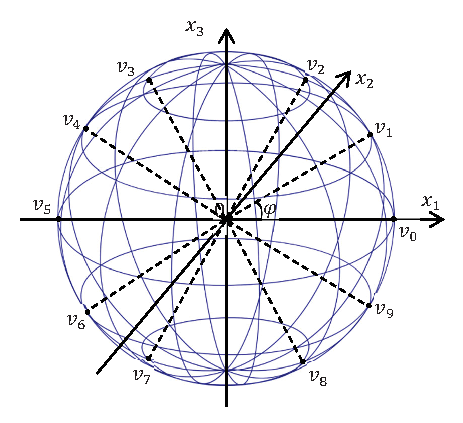
\includegraphics[scale=0.85]{./pic/sokol_Fig-1}
\bicaption{Построение точек валидационного множества $V$ на трехмерной сфере для $d=5$}
{Construction of points of the validation set $V$\break on the 
      three-dimensional sphere for $d=5$}
\label{pril:ris:fig1}
\end{wrapfigure}
    
Пусть в евклидовом пространстве ${\mathbb{R}^n}$ задана задача 
линейного программирования
\begin{equation*}
\bar x = \arg \max \left\{ {\left\langle {c,x} \right\rangle \mid {Ax \leqslant b,x \in {\mathbb{R}^n}} } \right\},\eqno(1)
\end{equation*}
где $c$ --- вектор коэффициентов целевой функции. Здесь и далее 
$\langle{\cdot, \cdot}\rangle$ обозначает скалярное произведение двух векторов. 
Обозначим $M = \left\{ {x \in {\mathbb{R}^n} \mid {Ax \leqslant b}} \right\}$~--- 
множество допустимых точек задачи~(1). По определению 
множество $M$ является выпуклым. Везде далее мы будем предполагать, что $M$ 
является непустым, ограниченным (и, следовательно, замкнутым) множеством, 
то есть задача~(1) имеет по крайней мере одно решение. 
Пусть $\tilde x \in {\mathbb{R}^n}$~--- приближенное решение 
задачи~(1), полученное с помощью некоторого
ЛП-решателя и требующее сертификации.

Идея метода валидации VaLiPro, описываемого в данной работе, заключается в 
построении конечного множества точек~$V$, покрывающих гиперсферу $S$ малого 
(по сравнению с размерами многогранника $M$) радиуса~$\rho$ с центром в точке 
сертифицируемого решения~$\tilde x$:
\begin{equation*}
V \subset S = \bigl\{ x \in \mathbb{R}^n \bigm\vert {{\left\| {x - \tilde x} \right\|}^2 = \rho ^2} \bigr\}.
\end{equation*}
\smallskip
\hrule
\bigskip
%
% ПРИМЕР 1. КОНЕЦ
%

\textbf{Рисунок~\ref{pril:ris:fig2}. Вставка серии рисунков.} 
Обращаем внимание авторов на проблему интеграции формул и шрифтов издательской
системы \LaTeXe{} в рисунки, созданные в графических редакторах или
иным способом. В подавляющем большинстве случаев авторы пытаются
разместить на своих рисунках формулы и надписи, которые выглядят
неестественно из-за того, что были набраны шрифтами, не входящими в
издательскую систему \LaTeXe{}.

Рассмотрим наиболее общий случай вставки в текст серии рисунков. 
Предполагаем, что автор выбрал оптимальный размер рисунков и на рисунках нет
надписей. 

1. Создается плавающий объект с помощью окружения
\begin{verbatim}
\begin{figure}{t!}
      ...
\end{figure}.
\end{verbatim}
Обязательные параметры \verb+{t}+ и \verb+{t!}+ задают размещение в верхней 
части страницы, \verb+{b}+ и \verb+{b!}+~--- в нижней части, 
а \verb+{h}+ и \verb+{h!}+~--- в том месте текста, где расположен плавающий объект.

\pagebreak
2. Внутри плавающего объекта создают окружение \verb!{picture}!
\begin{verbatim}
\begin{figure}{t!}
   \begin{picture}(170,65)
      ...
   \end{picture}
\end{figure}.
\end{verbatim}
В круглых скобках указывается размер резервируемой под рисунки области в миллиметрах.
В рассматриваемом примере ширина области равна 170~мм, а высота~--- 65~мм. Отметим,
что размер самих рисунков по высоте несколько меньше 65~мм.

3. С помощью команды \verb!\put(<x-координата>, <y-координата>){<объект>}! выполняют
размещение как самих рисунков, так и любых надписей в нужном месте зарезервированной 
области. 

Например, команда
\begin{verbatim}
      \put(11.3,7.5){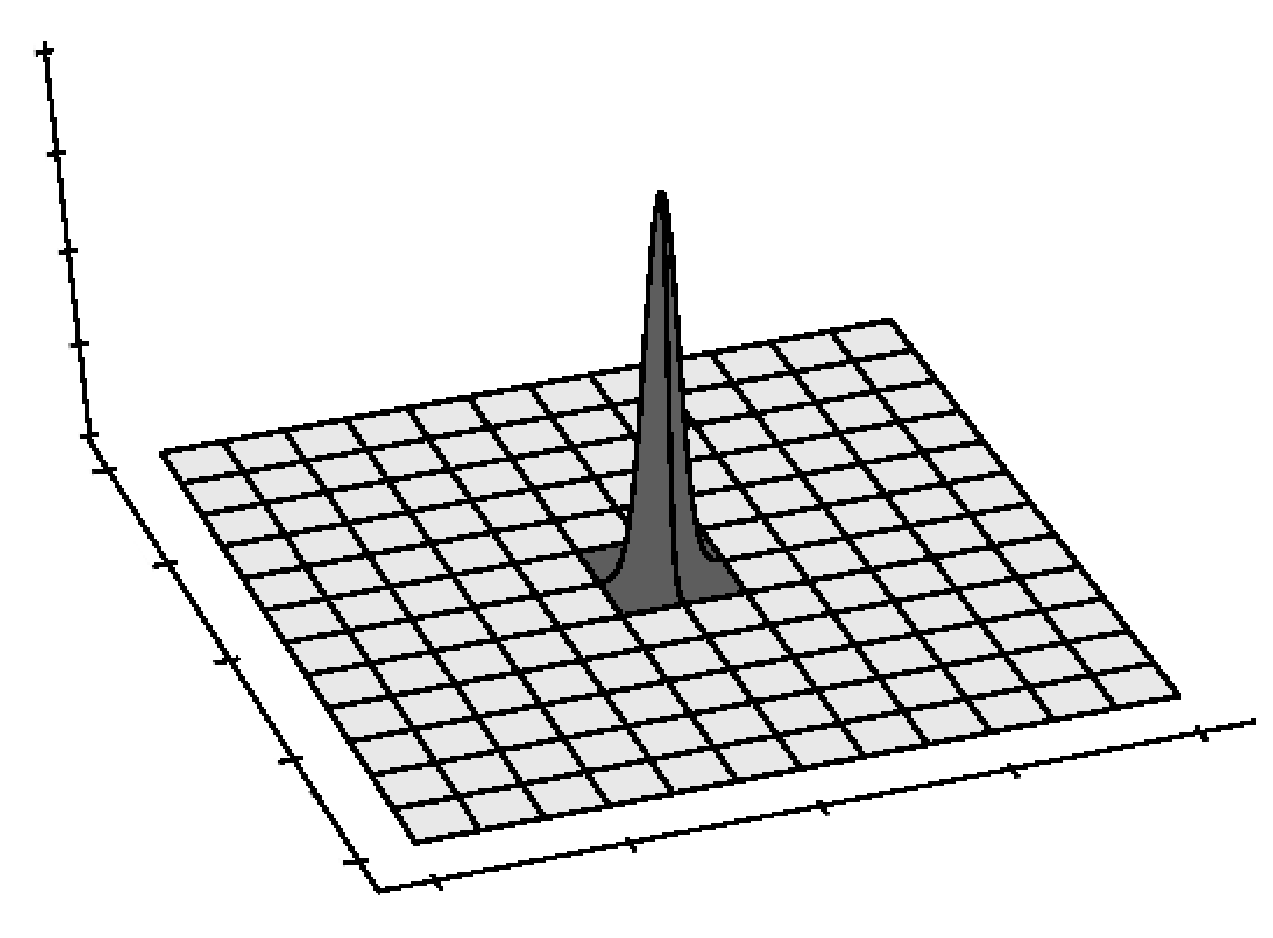
\includegraphics[width=70mm]{./pic/Bel_sol1r.eps}}
\end{verbatim}
загружает рисунок \verb!Bel_sol1r.eps! из директории \verb!./pic/!,
пропорционально масштабирует его до ширины 70~мм 
и помещает внутрь зарезервированной в окружении \verb!{picture}! области так, 
что координаты левого нижнего угла рисунка становятся равными 11.3~мм по
горизонтальной оси и 7.5~мм по вертикальной.

Команда \verb!\put(35,62){$u(x_1, x_2)$}! выводит поверх рисунка надпись $u(x_1, x_2)$.

В качестве объекта вывода команда \verb!\put(x,y)! может принимать окружение 
\verb!{picture}!:
\begin{verbatim}
      \put(x0,y0){\begin{picture}(0,0) ... \end{picture}}.
\end{verbatim}
Такое применение вложенных окружений \verb!{picture}! имеет смысл в случае,
если координаты второго рисунка и надписей на нем отличаются от координат
первого рисунка на вектор $(x0,y0)$. Размер области, резервируемой 
вложенным окружением \verb!{picture}!, не существенен и может быть \verb!(0,0)!.

Следующие команды выводят надписи на русском и английском языках поверх рисунка:
\begin{verbatim}
\put(75,43){\rotatebox{90}{Надпись}} 
\put(79,43){\rotatebox{90}{\contra{Legend}}}.
\end{verbatim}
Команда \verb!\contra{}! делает цвет шрифта серым.

4. После окружения \verb!{picture}! размещают подписи к рисункам с помощью
команды \verb!\bicaption!:
\begin{verbatim} 
\begin{figure}{t!}
      \begin{picture}(170,60)
      ...
      \end{picture}
      \bicaption{<текст подписи на русском языке>}{<текст подписи на английском языке>}
\end{figure}.
\end{verbatim}
%
% ПРИМЕР 2. ВСТАВКА РИСУНКОВ
%
\begin{figure}[t!]
\begin{picture}(170,65)\small
      \put(11.3,7.5){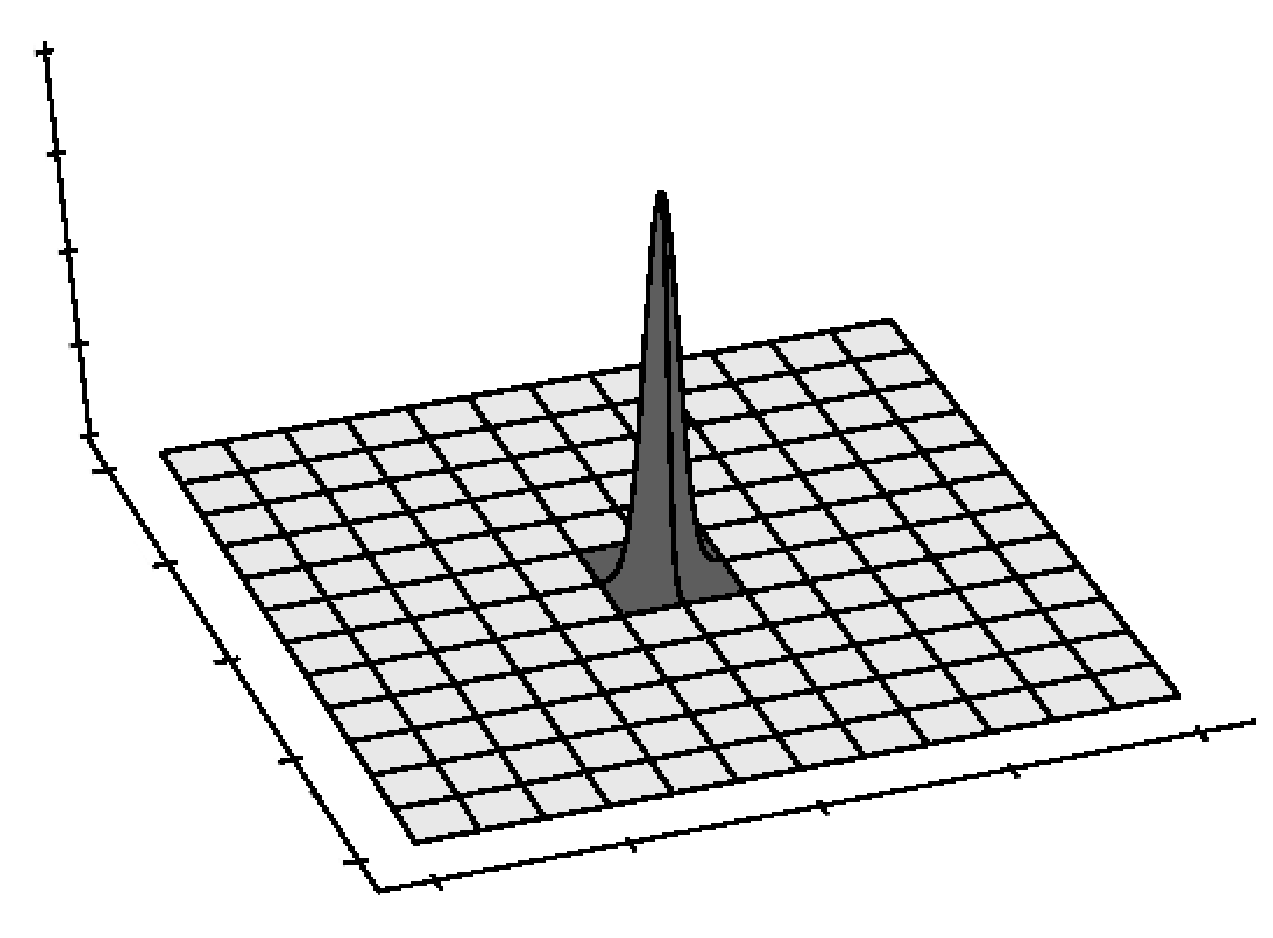
\includegraphics[width=70mm]{./pic/Bel_sol1r}}
      \put(35,62){$u(x_1, x_2)$}
      \put(6,55.5){$1.00$}
      \put(7,44){$0.50$}
      \put(8.3,34){$0.00$}
      \put(9,31){$0.50$}
      \put(15.7,20.5){$0.00$}
      \put(20.5,9){$-0.50$}
      \put(13,15){$x_2$}
      \put(31,6){$-0.50$}
      \put(55,10){$0.00$}
      \put(68,9){$x_1$}
      \put(77,14){$0.50$}
      \put(43,0){a)}
      \put(85,0){\begin{picture}(0,0)
            \put(11.3,7.5){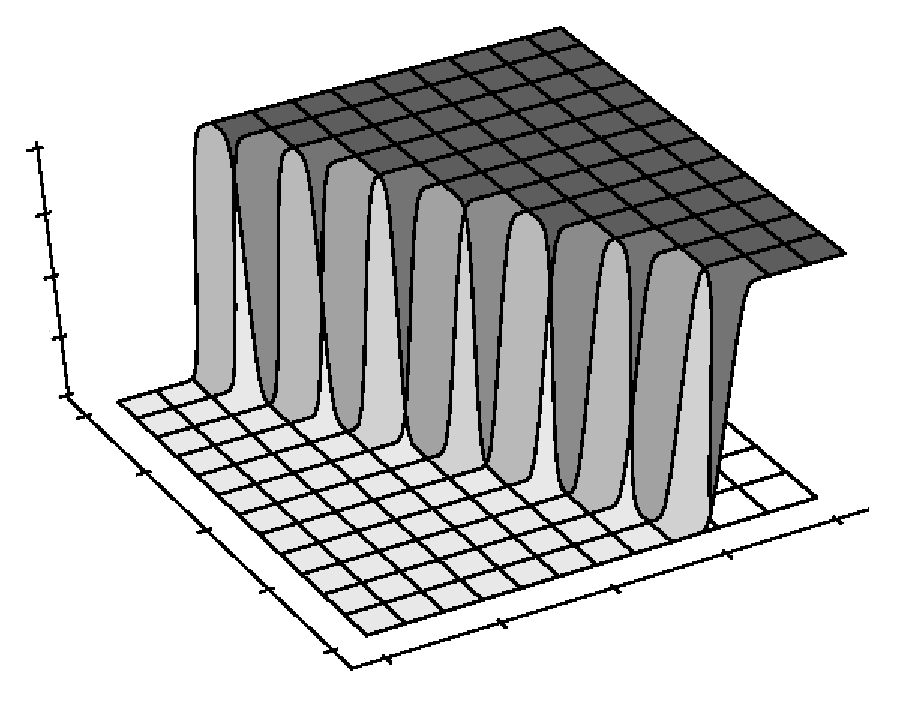
\includegraphics[width=70mm]{./pic/Bel_sol2r}}
            \put(25,62){$u(x_1, x_2)$}
            \put(5.5,49.5){$1.00$}
            \put(7,39){$0.50$}
            \put(8.3,30){$0.00$}
            \put(9.5,27){$1.00$}
            \put(19,18.5){$0.50$}
            \put(28.5,9){$0.00$}
            \put(16,13){$x_2$}
            \put(39.6,6){$0.00$}
            \put(58,11.5){$0.50$}
            \put(69,10){$x_1$}
            \put(75,17){$1.00$}
            \put(43,0){b)}
      \end{picture}}
      % надпись, повернутая на 90 градусов
      \put(75,43){\rotatebox{90}{Надпись}} % на русском языке
      \put(79,43){\rotatebox{90}{\contra{Legend}}} % на английском языке
\end{picture}
\bicaption{Точное решение: a) в примере~1.1 при $\beta = 1000$; b) в примере~1.2 при $\beta = 10^{-4}$}
      {Exact solution: a) in example~1.1 at $\beta = 1000$; b) in example~1.2 at $\beta = 10^{-4}$}
\label{pril:ris:fig2}
\end{figure}
%
% ПРИМЕР 2. КОНЕЦ
%

%============================ ПРИЛОЖЕНИЕ 3 ==================================
\newpage
\Appendix{Оформление таблиц}{pril:tbl}

\textbf{Таблица~\ref{pril:tbl:tab1}. Вставка текста на двух языках в ячейки таблицы.}
Представление информации в табличном виде часто используется при оформлении статей.
В простых случаях достаточно воспользоваться хорошо известными окружениями
\verb!{array}! и \verb!{tabular}!~[\ref{rfa:enlit:Kotelnikov}, \ref{rfa:enlit:Lvovski}].
Более удобными в применении являются окружение \verb!{tabularx}!~[\ref{rfa:enlit:Kotelnikov},
\ref{rfa:enlit:Samarin}] и команда \verb!\makecell!~[\ref{rfa:enlit:Lapko}].

Рассмотрим ключевые моменты при оформлении табл.~\ref{pril:tbl:tab1}. 
Заголовок таблицы на двух языках формируется командой \verb!\bicaption!.
В табл.~\ref{pril:tbl:tab1} имеется десять колонок, однако в первой строке таблицы
число колонок уменьшается до четырех за счет объединения трех колонок в одну
командой \verb!\multicolumn{3}{c|}{}!. Таблица задается окружением \verb!{tabularx}!
с параметрами:
\begin{verbatim}
\begin{tabularx}{170mm}{|>{\centering\arraybackslash}X|
      *{3}{>{\centering\arraybackslash}p{11mm}|}
      *{3}{>{\centering\arraybackslash}p{14mm}|}
      *{3}{>{\centering\arraybackslash}p{11mm}|}},
\end{verbatim}
где ширина таблицы задана равной ширине полосы (\verb!{170mm}!), 
первая колонка имеет неопределенную ширину (\verb!X!), за счет чего вся таблица выравнивается
по ширине в процессе компиляции, ширина остальных колонок задается явно в соответствующих
спецификаторах.

Для размещения внутри ячейки текста на две строки рекомендуем использовать команду
\verb!\makecell{}!, в которой команда \verb!\\! сохраняет свою функцию разбиения на строки.
Горизонтальная привязка задается в команде \verb!\makecell[]{}! с помощью необязательного
агрумента в квадратных скобках: 
\verb![t]!~--- привязка по верхней строке,
\verb![b]!~--- по нижней строке,
\verb![c]!~--- по центру блока.
Команда \verb!\contra{}! делает цвет шрифта серым.

%
% ПРИМЕР 1. ВСТАВКА ТАБЛИЦЫ
%
\begin{table}[h!]\small
\bicaption{Время выполнения в секундах программ на языке Fortran, NPB 3.3 класс D.}
      {Times in seconds of Fortran programs, NPB 3.3 class D}\label{pril:tbl:tab1}
\begin{tabularx}{170mm}{|>{\centering\arraybackslash}X|
      *{3}{>{\centering\arraybackslash}p{11mm}|}
      *{3}{>{\centering\arraybackslash}p{14mm}|}
      *{3}{>{\centering\arraybackslash}p{11mm}|}}
      \hline
      & \multicolumn{3}{c|}{\makecell{MPI программы\rlh\\ \contra{MPI programs}\rld}} 
      & \multicolumn{3}{c|}{\makecell{Преобразованные MPI программы\\ \contra{Converted MPI programs}}}  
      & \multicolumn{3}{c|}{\makecell{MPI программы + \textbf{FDVMH}\\ \contra{MPI programs + \textbf{FDVMH}}}} \\
      \COMMENT{
      & \multicolumn{3}{c|}{MPI программы} 
      & \multicolumn{3}{c|}{Преобразованные MPI программы}  
      & \multicolumn{3}{c|}{MPI программы + \textbf{FDVMH}} \\
      & \multicolumn{3}{c|}{\contra{MPI programs}} 
      & \multicolumn{3}{c|}{\contra{Converted MPI programs}}  
      & \multicolumn{3}{c|}{\contra{MPI programs + \textbf{FDVMH}}} \\
      }      
      \cline{2-10}
      & BT & CG & EP & BT & CG & EP & BT & CG & EP \\
      \hline
      \makecell[t]{1 узел\\ \contra{1 node}} & 665.1 & 397.5 & 93.68 & 785.29 & 376.8 & 83.34 & 63.3 & 80.99 & 0.62 \\
      \hline
      \makecell[c]{2 узла\\ \contra{2 nodes}} & 361.6 & 209.6 & 46.53 & 428.07 & 229.61 & 42.06 & 50.3 & 42.6  & 0.38 \\
      \hline
      \makecell[b]{4 узла\\ \contra{4 nodes}} & 196.8 & 91.3  & 23.3  & 232.36 & 96.67  & 25.16 & 45.5 & 34.3  & 0.17 \\
      \hline
\end{tabularx}
\end{table}
%
% ПРИМЕР 1. КОНЕЦ
%
  


\textbf{Таблица~\ref{pril:tbl:tab2}. Объединение нескольких вертикально расположенных 
ячеек в одну.} В следующей таблице показано применение команды 
\begin{verbatim}
            \multirow[<vpos>]{<rows>}[<bigstruts>]{<width>}[<vmove>]{<text>}.
\end{verbatim}
В примере используются только обязательные аргументы 
\verb!{<rows>}!, \verb!{<width>}! и \verb!{<text>}! [\ref{rfa:enlit:mrow}].


%
% ПРИМЕР 2. ВСТАВКА ТАБЛИЦЫ
%
\begin{table}[h!]
\bicaption{Результаты численных экспериментов в примере~1.1}
      {Results of numerical experiments in example~1.1}
\label{pril:tbl:tab2}
\small
\renewcommand{\tabcolsep}{2pt}
\begin{tabularx}{170mm}{|%
            >{\centering\arraybackslash}p{5mm} |
            >{\centering\arraybackslash}p{16mm} ||
            >{\centering\arraybackslash}p{21mm} |
            >{\centering\arraybackslash}p{12mm} |
            >{\centering\arraybackslash}p{21mm} |
            >{\centering\arraybackslash}p{12mm} ||
            >{\centering\arraybackslash}p{21mm} |
            >{\centering\arraybackslash}p{12mm} |
            >{\centering\arraybackslash}p{21mm} |
            >{\centering\arraybackslash} X |
      }
      \hline
      \multirow{4}{*}{$K$} &  
      \multirow{4}{*}{$N$$\times$$N$} & 
      \multicolumn{2}{c|}{\makecell{МКР\rlh\\ \contra{FDM}\rld}} & 
      \multicolumn{2}{c||}{\makecell{метод КНК\\ \contra{LSC method}}} & 
      \multicolumn{2}{c|}{\makecell{МКР\\ \contra{FDM}}} & 
      \multicolumn{2}{c|}{\makecell{метод КНК\\ \contra{LSC method}}} \\
      \cline{3-10}
      &
      &
      $\|E_a\|_{\infty}$\rl &
      $R$ &
      $\|E_a\|_{\infty}$ &
      $R$ &
      $\|E_a\|_{\infty}$ &
      $R$ &
      $\|E_a\|_{\infty}$ &
      $R$ \\
      \cline{3-10}
      & & \multicolumn{4}{c||}{$\beta = 100$} & \multicolumn{4}{c|}{$\beta = 1000$} \\
      \hline
      \multirow{4}{*}{$2$} & 10$\times$10 & $3.843 \cdot 10^{-1}$ & --- 	 & $2.92 \cdot 10^{-1}$ & ---    & $19.978$ 			 & --- 	  & $2.23$               & --- \\
      & 20$\times$20 & $6.771 \cdot 10^{-2}$ & $2.50$ & $5.85 \cdot 10^{-2}$ & $2.31$ & $3.11$ 			     & $2.68$ & $7.74 \cdot 10^{-1}$ & $1.52$\\
      & 40$\times$40 & $1.591 \cdot 10^{-2}$ & $2.09$ & $1.38 \cdot 10^{-2}$ & $2.08$ & $1.959 \cdot 10^{-1}$ & $3.99$ & $1.64 \cdot 10^{-1}$ & $2.23$\\
      & 80$\times$80 & $3.921 \cdot 10^{-3}$ & $2.02$ & $3.45 \cdot 10^{-3}$ & $2.00$ & $4.104 \cdot 10^{-2}$ & $2.25$ & $3.55 \cdot 10^{-2}$ & $2.20$\\
      \hline
\COMMENT{
      \multirow{4}{*}{$6$}	
      & 10$\times$10 & $4.942 \cdot 10^{-3}$ & ---    & $7.11 \cdot 10^{-4}$ & ---    & $7.985$ 			    & --- 	 & $2.46 \cdot 10^{-1}$ & ---  \\
      & 20$\times$20 & $3.594 \cdot 10^{-5}$ & $7.10$ & $7.30 \cdot 10^{-6}$ & $6.60$ & $1.13 \cdot 10^{-1}$  & $6.14$ & $1.71 \cdot 10^{-2}$ & $3.84$\\
      & 40$\times$40 & $4.635 \cdot 10^{-7}$ & $6.28$ & $8.65 \cdot 10^{-8}$ & $6.39$ & $7.624 \cdot 10^{-4}$ & $7.21$ & $1.44 \cdot 10^{-4}$ & $6.89$\\
      & 80$\times$80 & $7.110 \cdot 10^{-9}$ & $6.03$ & $1.23 \cdot 10^{-9}$ & $6.13$ & $8.193 \cdot 10^{-6}$ & $6.54$ & $1.61 \cdot 10^{-6}$ & $6.48$\\
      \hline	
      \multirow{4}{*}{$10$} 
      & 10$\times$10 & $3.036 \cdot 10^{-3}$ & --- 	 & $7.37 \cdot 10^{-7}$  & ---     & $2.936$               & --- 	   & $1.51 \cdot 10^{-2}$  & ---\\
      & 20$\times$20 & $9.894 \cdot 10^{-7}$ & $11.58$ & $4.81 \cdot 10^{-10}$ & $10.58$ & $3.086 \cdot 10^{-1}$ & $3.25$  & $8.76 \cdot 10^{-5}$  & $7.42$\\
      & 40$\times$40 & $8.473 \cdot 10^{-10}$& $10.19$ & $3.54 \cdot 10^{-13}$ & $10.40$ & $1.559 \cdot 10^{-4}$ & $10.95$ & $5.93 \cdot 10^{-8}$  & $10.52$\\
      & 80$\times$80 & $8.407 \cdot 10^{-13}$& $9.98$  & $7.52 \cdot 10^{-14}$ & $2.23$  & $8.78  \cdot 10^{-8}$ & $10.79$ & $7.75 \cdot 10^{-11}$ & $9.57$\\
      \hline	
      \multirow{5}{*}{$18$} 
      & 5$\times$5   & ---  & --- 	 & $1.74 \cdot 10^{-8}$  & ---     & ---				   & --- 	 & $1.03$  & ---\\
      & 10$\times$10 & $8.388 \cdot 10^{-2}$ & --- 	 & $1.43 \cdot 10^{-13}$ & $13.57$ & $154283$              & --- 	 & $2.91 \cdot 10^{-5}$ & $15.11$\\
      & 20$\times$20 & $2.844 \cdot 10^{-7}$ & $18.17$ & $3.04 \cdot 10^{-14}$ & $2.23$  & $307.82$              & $8.97$  & $1.08 \cdot 10^{-9}$ & $14.71$\\
      & 40$\times$40 & $1.826 \cdot 10^{-12}$& $17.25$ & ---					 &  ---    & $1.19  \cdot 10^{-3}$ & $17.98$ & $4.33 \cdot 10^{-13}$	 & $11.28$\\
      & 80$\times$80 & $2.992 \cdot 10^{-12}$& $-0.71$ & ---					 &  ---    & $3.92  \cdot 10^{-9}$ & $18.21$ & ---					 &  ---\\
      \hline	
}% COMMENT
\end{tabularx}
\end{table}
%
% ПРИМЕР 2. КОНЕЦ
%
              
      
%============================ ПРИЛОЖЕНИЕ 4 ==================================
\newpage
\Appendix{Оформление списка литературы}{pril:spis}
\setcounter{rulitcnt}{0}


\medskip
Книги:

\rlitem{VVVVVV}{%
\textit{Воеводин В.В., Воеводин Вл.В.}
Параллельные вычисления. СПб.: БХВ--Петербург, 2002.
}

\rlitem{Belyaevrus:Fedorenko1994}{%
\textit{Федоренко Р.П.} 
Введение в вычислительную физику. 
М.: Московский физико-технический институт, 1994.}

\rlitem{LLM}
{\textit{Ландау Л.Д., Лифшиц Е.М.} Теоретическая физика. Т. 1. Механика.
 М.: Наука, 1973.}


\medskip
Статьи:

\rlitem{Algo500}{%
\textit{Antonov A.S., Nikitenko D.A., Voevodin V.V.}
Algo500~--- a new approach to the joint analysis of algorithms and computers~// 
Lobachevskii J. Math. 2020. \textbf{41}, N~8. 1435--1443.
\doi{10.1134/S1995080220080041}.
}

\rlitem{Belyaevrus:Isaev2010}{%
\textit{Исаев В.И., Шапеев В.П.} Варианты метода коллокаций и наименьших
квадратов повышенной точности для численного решения уравнений 
Навье--Стокса~// Журнал вычислительной математики и математической физики.
2010. {\bf 50}, \No~10. 1758--1770. 
\url{https://www.elibrary.ru/item.asp?id=15249920}}

\rlitem{Belyaevrus:Vorozhtsov2019}{%
\textit{Vorozhtsov E.V., Shapeev V.P.} On the efficiency of combining
different methods for acceleration of iterations at the solution of PDEs by
the method of collocations and least residuals~//
Applied Mathematics and Computation. 2019. {\bf 363}. 1--19. 
\doi{10.1016/j.amc.2019.124644}.
%\url{https://www.sciencedirect.com/science/article/abs/pii/S0096300319306368}.
}

\rlitem{Belyaevrus:Shapeev2021}{%
\textit{Shapeev V.P., Golushko S.K., Belyaev V.A., Bryndin L.S., Kirillov P.I.}
New versions of the least-squares collocation method for solving differential 
and integral equations~// Journal of Physics: Conference Series. 2021. 
{\bf 1715}, N~012031. 1--8. \doi{10.1088/1742-6596/1715/1/012031}.
%\url{https://iopscience.iop.org/article/10.1088/1742-6596/1715/1/012031}.
}

\rlitem{sokol_15}{%
\textit{Панюков А.В., Горбик В.В.} 
Применение массивно-параллельных вычислений для решения задач линейного 
программирования с абсолютной точностью~// 
Автоматика и телемеханика. 2012. \No~2. 73--88.
}


\medskip
Труды конференций:

\rlitem{GPU-faster}{%
\textit{Бахтин В.А., Колганов А.С., Крюков В.А., Поддерюгина Н.В., 
Притула М.Н.} 
Методы динамической настройки DVMH-программ на кластеры с ускорителями~// 
Труды Международной конференции ``Суперкомпьютерные дни в России 2015'', 
28--29~сентября 2015, Москва.
М.: Изд-во Моск. гос. ун-та, 2015. 257--269.}

\rlitem{polly-reduction}{%
\textit{Doerfert J., Streit K., Hack S., Benaissa Z.} 
Polly's polyhedral scheduling in the presence of reductions~// Proc.
5th Int. Workshop on Polyhedral Compilation Techniques (IMPACT 2015), 
January~19, 2015, Amsterdam, The Netherlands.
\url{https://citeseerx.ist.psu.edu/viewdoc/download?doi=10.1.1.1054.1804&rep=rep1&type=pdf}.
}

\medskip
Интернет-ресурсы:

\rlitem{openmp-status}{%
Компиляторы и инструменты OpenMP. 
\url{https://www.openmp.org/resources/openmp-compilers-tools/}. 
(Дата обращения: 15 октября 2021).
}

\rlitem{nas}{%
NAS Parallel Benchmarks. 
\url{https://www.nas.nasa.gov/publications/npb.html}.
(Дата обращения: 15 октября 2021).}

\rlitem{CUDA}{%
NVidia CUDA Zone. 
\url{https://developer.nvidia.com/cuda-zone}.
(Дата обращения: 10 ноября 2021).
}


\medskip
Другие ресурсы:

\rlitem{sokol_21}{%
\textit{Соколинский Л.Б.} 
Параллельный программный каркас BSF. 
Свидетельство о государственной регистрации программы для ЭВМ 2020661344, 
22.09.2020.}



%============================ ПРИЛОЖЕНИЕ 5 ==================================
\newpage
\Appendix{Оформление References}{pril:refer}
\setcounter{enlitcnt}{0}

\medskip
Книги:

\elitem{i8}{%
V.~V.~Voevodin and Vl.~V.~Voevodin, {\it The Parallel Computing}
(BHV-Petersburg, St. Petersburg, 2002) [in Russian].}

\elitem{i13}{%
R.~P.~Fedorenko, \textit{Introduction to Computational Physics} 
(Moscow Inst. Phys. Technol., Moscow, 1994) [in Russian].}

\elitem{i3}{%
L.~D.~Landau and E.~M.~Lifshitz, 
{\it Course of Theoretical Physics}, Vol.~1: {\it Mechanics}
(Nauka, Moscow, 1973; Pergamon, Oxford, 1977).}


\medskip
Статьи:

\elitem{i5}{%
A.~S.~Antonov, D.~A.~Nikitenko, and V.~V.~Voevodin, 
``Algo500~--- A New Approach to the Joint Analysis of Algorithms and Computers,’’ 
Lobachevskii J. Math. \textbf{41}~(8), 1435--1443 (2020).
\doi{10.1134/S1995080220080041}.
}

\elitem{i1}{%
V.~I.~Isaev and V.~P.~Shapeev, ``High-Accuracy Versions of the Collocations 
and Least Squares Method for the Numerical Solution of the Navier--Stokes 
Equations,’’
Zh. Vychisl. Mat. Mat. Fiz. {\bf 50} (10), 1758--1770 (2010) 
 [Comput. Math. Math. Phys. {\bf 50} (10), 1670--1681 (2010).
\doi{10.1134/S0965542510100040}].
}

\elitem{i2}{%
E.~V.~Vorozhtsov and V.~P.~Shapeev, ``On the Efficiency of Combining Different 
Methods for Acceleration of Iterations at the Solution of PDEs by the Method of 
Collocations and Least Residuals,'' Appl. Math. Comput. {\bf 363} (2019). 
\doi{10.1016/j.amc.2019.124644}. 
}

\elitem{i8}{%
V.~P.~Shapeev, S.~K.~Golushko, V.~A.~Belyaev, et al., 
``New Versions of the Least-Squares Collocation Method for Solving 
Differential and Integral Equations,'’
  J. Phys.: Conf. Ser. {\bf 1715} (2021), 1--8.
\doi{10.1088/1742-6596/1715/1/012031}. 
}

\elitem{i15}{%
A.~V.~Panyukov and V.~V.~Gorbik, ``Using Massively Parallel Computations for Absolutely Precise Solution of the Linear Programming Problems,’’
  Avtom. Telemekh., No.~2, 73--88 (2012)
  [Autom. Rem. Contr. \textbf{73}~(2), 276--290 (2012). 
  \doi{10.1134/S0005117912020063}].
}


\medskip
Труды конференций:

\elitem{i24}{%
V.~Bakhtin, A.~Kolganov, V.~Krukov, et al.,
``Dynamic Tuning Methods of DVMH-Programs for Clusters with Accelerators,’’
in {\it Proc. Int. Conf. on Russian Supercomputing Days, Moscow, Russia,
September~28--29, 2015}
(Mosk. Gos. Univ., Moscow, 2015), pp.~257--269.
}

\elitem{i23}{%
J.~Doerfert, K.~Streit, S.~Hack, and Z.~Benaissa,
``Polly’s Polyhedral Scheduling in the Presence of Reductions,''
  in {\it Proc. 5th Int. Workshop on Polyhedral Compilation Techniques (IMPACT 2015),
  Amsterdam, The Netherlands, January~19, 2015},
\url{https://citeseerx.ist.psu.edu/viewdoc/download?doi=10.1.1.1054.1804&rep=rep1&type=pdf}. 
Cited October~15, 2021.
}

\medskip
Интернет-ресурсы:

\elitem{i6}{%
OpenMP Compilers \& Tools. 
\url{https://www.openmp.org/resources/openmp-compilers-tools/}. 
Cited October~15, 2021.
}

\elitem{i15}{%
NAS Parallel Benchmarks. 
\url{https://www.nas.nasa.gov/publications/npb.html}.
Cited October 15, 2021.
}

\elitem{iii}{%
NVidia CUDA Zone. 
\url{https://developer.nvidia.com/cuda-zone}. 
Cited November 15, 2020.}


\medskip
Другие ресурсы:

\elitem{i21}{%
L.~B.~Sokolinsky, {\it Parallel Algorithmic Skeleton BSF},
  Certificate of RF Registration of Computer Program No.~2 020 661 344.
Date of Registration: September 22, 2020. 
}





%============================ ПРИЛОЖЕНИЕ 6 ==================================
\newpage\nolinenumbers
%
% ПРИЛОЖЕНИЕ 4
% используйте как шаблон письма в редакцию
%
\thispagestyle{empty}
%
% Следующие две строки нужно убрать
%
\Appendix{Сопроводительное письмо в редакцию}{pril:sopr}


{\large
\hfill\parbox[t]{70mm}{
Заместителю главного редактора\\
научного журнала\\[2mm]
``Вычислительные методы и\\
программирование''\\[2mm]
д.ф.-м.н. А. В. Смирнову
}
\vspace*{12mm}
\begin{center}
СОПРОВОДИТЕЛЬНОЕ ПИСЬМО
\end{center}

\vspace*{3mm}

Просим опубликовать в журнале ``Вычислительные методы и программирование'' статью 
``<НАЗВАНИЕ СТАТЬИ>''.

Сообщаем следующую информацию о каждом авторе статьи.

1. Фамилия, имя, отчество полностью (с написанием на английском языке).

2. Основное место работы полностью с указанием полного почтового адреса и URL сайта организации (с переводом на английский язык).

3. Должность по основному месту работы (с переводом на английский язык).

4. Ученая степень и ученое звание (с переводом на английский язык).

5. Телефон служебный, домашний и мобильный.

6. E-mail.

7. ORCID (\corr{обязательно}; если еще не получен, посетите \url{https://orcid.org/register}).

8. Номер и название рубрики ГРНТИ (только для статей на русском) и код OECD для подаваемой статьи.

9. Желательно: ссылки на профили авторов в elibrary.ru для упрощения и корректности подлинковки статьи.

\vspace*{2mm}
Текущую переписку по вопросам публикации статьи следует вести с <Фамилия И.О.>.

\vspace*{2mm}
Авторы согласны с правилами подготовки статьи к публикации, включая рецензирование, 
научное и литературное редактирование и доведение статьи до редакторских стандартов, 
принятых в рамках журнала.

Авторы ознакомлены с Публикационной этикой журнала и согласны с ее положениями.

Авторы также согласны с передачей журналу своего права на издание и распространение 
статьи в электронной и бумажной версиях, в том числе на размещение библиографической 
информации о статье в Российском индексе научного цитирования (РИНЦ) и в других базах 
научного цитирования и на размещение полных текстов статей в Научной электронной 
библиотеке (elibrary.ru) и портале http://www.mathnet.ru для свободного доступа всем пользователям Интернет независимо от их категории и местоположения.

\vspace*{15mm}
<Дата>\hfill\parbox[t]{70mm}{\hrulefill~<И.О. Фамилия>}

\vspace*{8mm}

\hfill\parbox[t]{70mm}{\hrulefill~<И.О. Фамилия>}

}%large



\end{document}

